\documentclass[a4paper,12pt]{article}

% --- Шрифты и кодировки ---
\usepackage[utf8]{inputenc}
\usepackage[T1]{fontenc}
\usepackage[russian]{babel}
\usepackage{mathptmx} % Times New Roman

% --- Поля ---
\usepackage[left=3cm, right=1.5cm, top=2cm, bottom=2cm]{geometry}

% --- Межстрочный интервал ---
\usepackage{setspace}
\onehalfspacing % Интервал 1.5

% --- Абзацы ---
\setlength{\parindent}{1.25cm} % Красная строка
\setlength{\parskip}{0pt}      % Без межабзацного отступа

% --- Графика и вёрстка ---
\usepackage{graphicx}
\usepackage{pgfplots}
\pgfplotsset{compat=1.18}
\usepackage{svg}
\usepackage{float}
\usepackage{qrcode}

% --- Математика ---
\usepackage{amsmath}

% --- Программный код ---
\usepackage{minted}
% \usepackage{listings}
% \lstset{
%     language=Python,
%     basicstyle=\ttfamily\small,
%     numbers=left,
%     numberstyle=\tiny,
%     stepnumber=1,
%     numbersep=5pt,
%     frame=single,
%     breaklines=true,
%     showstringspaces=false,
%     tabsize=4
% }

% --- Прочее ---
\usepackage{titling}
\usepackage{enumitem}
\usepackage{tocloft}
\renewcommand{\cftsecleader}{\cftdotfill{\cftdotsep}}

% --- Гиперссылки ---
\usepackage[hidelinks]{hyperref}

\begin{document}

\tableofcontents

\newpage

\section{Введение}
Процессы переноса примесей и тепла в жидких средах представляют собой актуальную задачу как для теоретических исследований в области гидродинамики, так и для различных прикладных применений. В данной лабораторной работе рассматривается численное моделирование распространения пассивного скалярного поля — такого, как концентрация вещества или температура — в условиях стационарного двумерного течения.
Исследование проводится на основе упрощённой физической модели: анализируется поведение примеси на поверхности жидкости в ограниченном пространстве (например, в условном "бассейне"), где заранее задано устойчивое течение. Основное внимание уделяется изучению того, как распределение концентрации изменяется во времени и в пространстве под влиянием этого течения.
Цель работы — построение и исследование решения двумерного уравнения переноса с заданными начальными и граничными условиями, позволяющее определить, как изменяется концентрация примеси в заданной точке или области спустя определённый промежуток времени.

\newpage

\section{Формализация задачи}

В данной работе задача моделирования переноса пассивной примеси в двумерном стационарном течении формализуется через набор сущностей, каждая из которых обладает определёнными характеристиками и моделируется с использованием допущений, упрощающих физическую постановку.

\subsection{Скалярное поле концентрации}

\textbf{Обозначение:}  
\begin{itemize}
    \item $C(x, y, t)$ — значение концентрации (или температуры) в точке пространства в момент времени $t$
\end{itemize}
Характеристики:
\begin{itemize}
    \item Измеряется в условных единицах концентрации (масса/объем, температура и т.п.);
    \item Является функцией пространства и времени;
    \item Переносится потоком без изменения при движении материальной точки (пассивация).
\end{itemize}
Допущения:
\begin{itemize}
    \item Примесь не влияет на течение и не взаимодействует с другими примесями;
    \item Диффузия не учитывается (чистый конвективный перенос);
    \item Нет источников и стоков примеси в области моделирования.
\end{itemize}


\subsection{Чaстицы}
\textbf{Обозначение:}  
\begin{itemize}
    \item $(x(t), y(t))$ — координаты частицы во времени
\end{itemize}
Характеристики:
\begin{itemize}
    \item Определяется решением системы ОДУ:  
    \[
    \begin{cases}
    \frac{dx}{dt} = u(x,y), \\
    \frac{dy}{dt} = v(x,y);
    \end{cases}
    \]
    \item Отражает путь, по которому движется материальная точка в поле скоростей;
    \item Используется для вычисления переноса величины $C$.
\end{itemize}
Допущения:
\begin{itemize}
    \item Частицы не взаимодействуют друг с другом;
    \item Не происходит разделения или слияния траекторий;
    \item Интеграция осуществляется с помощью метода Эйлера первого порядка.
\end{itemize}

\subsection{Начальное распределение}
\textbf{Обозначение:}  
\begin{itemize}
    \item $C_0(x, y)$ — значение концентрации в начальный момент времени $t = 0$
\end{itemize}
Характеристики:
\begin{itemize}
    \item Задает стартовое состояние моделируемого поля;
    \item Может быть аналитической функцией или численно заданным полем;
    \item Определяет начальные условия для всех частиц.
\end{itemize}
Допущения:
\begin{itemize}
    \item Распределение известно заранее и не содержит шумов или погрешностей;
    \item На границах области значения вне диапазона могут игнорироваться (в зависимости от схемы граничных условий);
    \item Вне заданной области начальная концентрация считается равной нулю, если не указано иное.
\end{itemize}


\newpage

\section{Cоставление математической модели}

Основу анализа переноса пассивных примесей в движущейся жидкости составляет уравнение конвективного переноса. В двумерной постановке, рассматриваемой в данной работе, это уравнение имеет следующий вид: 

$$
\frac{\partial C}{\partial t} + u(x,y)\frac{\partial C}{\partial x} + v(x,y)\frac{\partial C}{\partial y} = 0
$$
где:
\begin{itemize}
\item $t$ — время,
\item $x, y$ — пространственные координаты, 
\item $C = C(x,y,t)$ — скалярная величина, характеризующая концентрацию вещества или температуру,
\item $u(x,y), v(x,y)$ — компоненты поля скоростей вдоль осей $x$ и $y$ соответственно.
\end{itemize}

Начальное состояние скалярного поля задаётся функцией распределения:
$C(x,y,0) = C_0(x,y).$

Для описания скорости движения жидкости используется функция тока $\psi(x,y)$, с помощью которой компоненты скорости определяются следующим образом:

$$
\begin{cases}
u(x,y) = -\frac{\partial \psi}{\partial y},\\
v(x,y) = \frac{\partial \psi}{\partial x}.
\end{cases}
$$

Задача математического моделирования заключается в нахождении распределения $C(x,y,t)$ во времени и пространстве на основе известных начальных условий и заданного характера течения.

Для численного решения применяется лагранжев подход, также известный как метод трассировки частиц. В его основе лежит предположение, что каждая частица переносит с собой неизменное значение $C$ вдоль своей траектории. Движение частиц описывается системой обыкновенных дифференциальных уравнений:

$$
\begin{cases}
\frac{dx}{dt} = u(x,y),\\
\frac{dy}{dt} = v(x,y).
\end{cases}
$$

Численная интеграция осуществляется с использованием метода Эйлера первого порядка:

$$
\begin{cases}
x^{n+1} = x^n + u(x^n, y^n) \cdot \Delta t,\\
y^{n+1} = y^n + v(x^n, y^n) \cdot \Delta t,
\end{cases}
$$

где $\Delta t$ — шаг по времени, а верхние индексы $n$ и $n+1$ обозначают номера временных шагов. Распределение концентрации в любой момент времени определяется с помощью интерполяции значений, переносимых частицами, траектории которых были рассчитаны.

\newpage


\section{Численные эксперименты}

В данном разделе для решения задачи переноса пассивной примеси применяются и сравниваются два различных численных подхода: лагранжев (метод частиц) и эйлеров (метод конечных разностей).

\subsection{Описание численных методов}

\subsubsection{Метод частиц (Лагранжев подход)}
Данный метод основан на отслеживании траекторий большого ансамбля отдельных частиц, каждая из которых несет постоянное значение концентрации. Движение частиц определяется полем скоростей и рассчитывается путем интегрирования системы обыкновенных дифференциальных уравнений:
$$
\begin{cases}
    \frac{dx}{dt}=u(x,y), \\
    \frac{dy}{dt}=v(x,y).
\end{cases}
$$
Для численного интегрирования этой системы в нашей реализации был использован метод Рунге-Кутты 4-го порядка, обеспечивающий высокую точность расчета траекторий. Значение концентрации в узлах регулярной сетки в любой момент времени получается путем интерполяции значений, переносимых частицами. Основное преимущество данного подхода — отсутствие численной диффузии, что позволяет моделировать перенос с сохранением резких градиентов.

\subsubsection{Метод конечных разностей (Эйлеров подход)}
В отличие от лагранжева подхода, эйлеров метод рассматривает изменение концентрации в фиксированных точках пространства (узлах сетки). Исходное уравнение в частных производных аппроксимируется системой конечно-разностных уравнений. В данной работе была применена явная схема с аппроксимацией производной по времени методом Эйлера первого порядка, а пространственные производные аппроксимировались с помощью \textbf{противопотоковой схемы первого порядка (Upwind scheme)}. Эта схема выбирает разность "против потока" для устойчивого решения уравнений гиперболического типа.

Недостатком данной простой схемы является ее подверженность \textbf{численной диффузии} — искусственному "размыванию" резких градиентов, которое вносится самой схемой аппроксимации.

\subsection{Результаты и сравнение}
Для сравнения методов было проведено моделирование переноса начального распределения концентрации до момента времени $t=0.4$. Ниже представлены результаты для начального состояния и для временных срезов $t=0.1, 0.2, 0.3, 0.4$.

\begin{figure}[H]
    \centering
    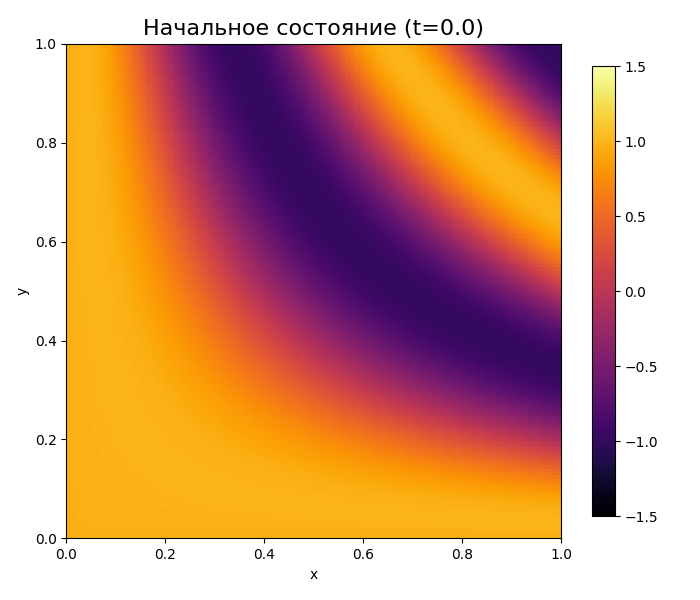
\includegraphics[width=0.6\textwidth]{comparison_results/initial_state.png}
    \caption{Начальное распределение концентрации C(x,y,0) в момент времени t=0.0.}
    \label{fig:initial}
\end{figure}

% --- Сравнение для t=0.1 ---
\begin{figure}[H]
    \centering
    \begin{minipage}{0.49\textwidth}
        \centering
        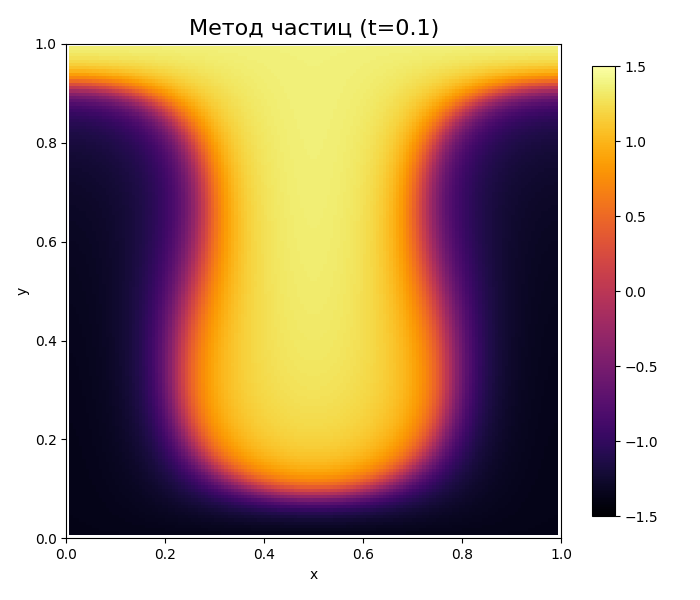
\includegraphics[width=\linewidth]{comparison_results/particle_method_t_0.1.png}
    \end{minipage}
    \hfill
    \begin{minipage}{0.49\textwidth}
        \centering
        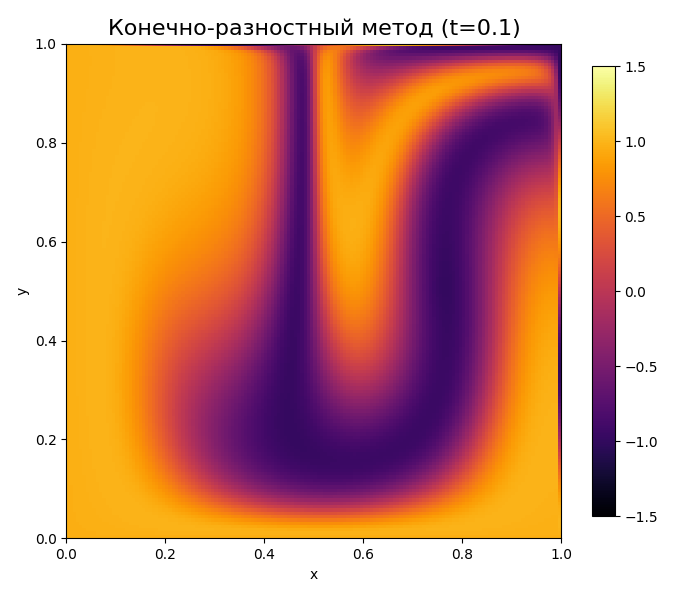
\includegraphics[width=\linewidth]{comparison_results/fdm_method_t_0.1.png}
    \end{minipage}
    \caption{Сравнение результатов в момент времени t=0.1. Слева — метод частиц, справа — конечно-разностный метод.}
    \label{fig:t01}
\end{figure}

% --- Сравнение для t=0.2 ---
\begin{figure}[H]
    \centering
    \begin{minipage}{0.49\textwidth}
        \centering
        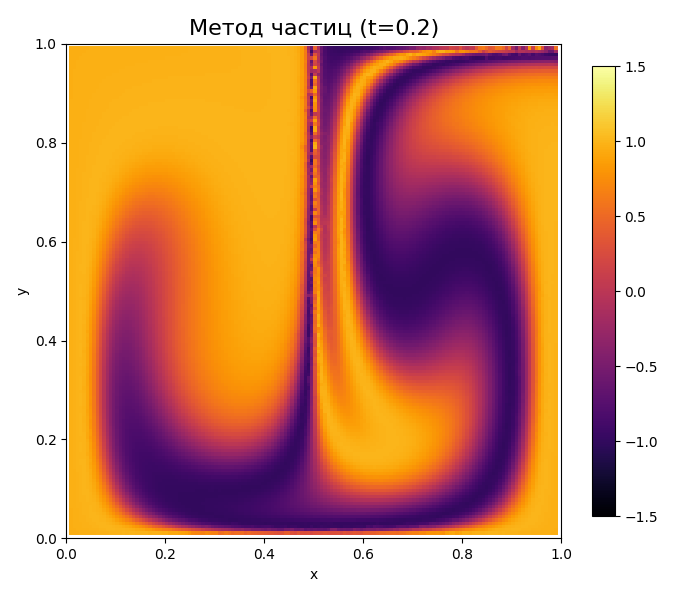
\includegraphics[width=\linewidth]{comparison_results/particle_method_t_0.2.png}
    \end{minipage}
    \hfill
    \begin{minipage}{0.49\textwidth}
        \centering
        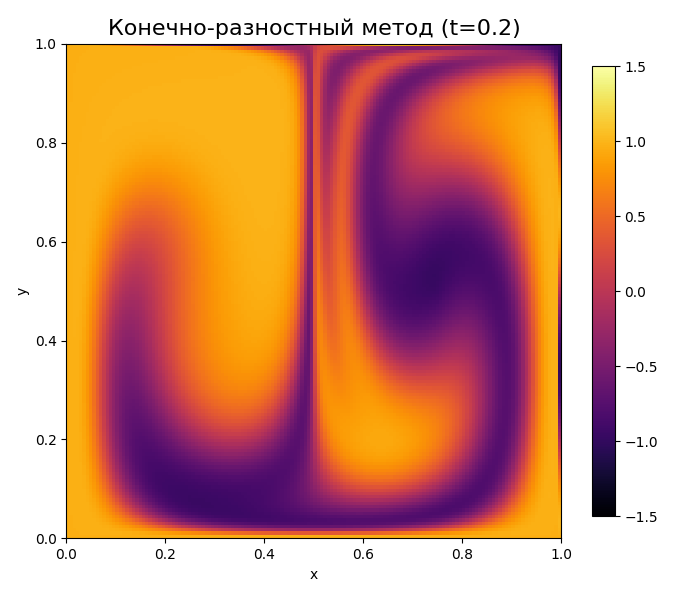
\includegraphics[width=\linewidth]{comparison_results/fdm_method_t_0.2.png}
    \end{minipage}
    \caption{Сравнение результатов в момент времени t=0.2. Слева — метод частиц, справа — конечно-разностный метод.}
    \label{fig:t02}
\end{figure}

% --- Сравнение для t=0.3 ---
\begin{figure}[H]
    \centering
    \begin{minipage}{0.49\textwidth}
        \centering
        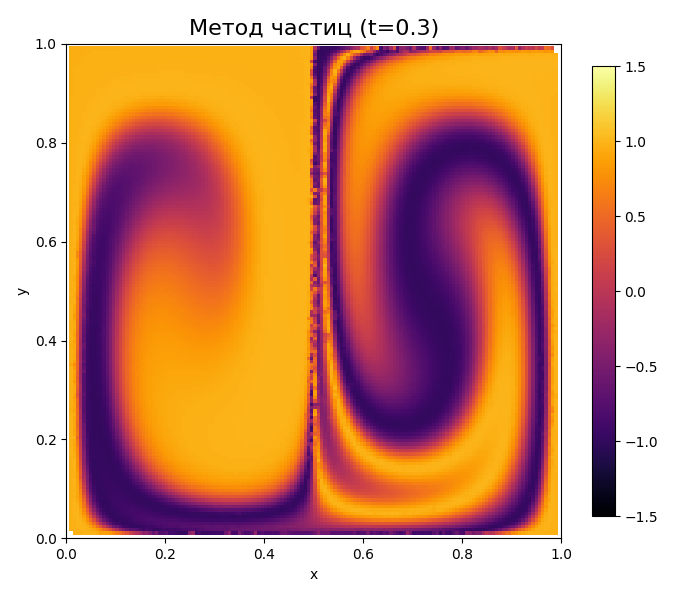
\includegraphics[width=\linewidth]{comparison_results/particle_method_t_0.3.png}
    \end{minipage}
    \hfill
    \begin{minipage}{0.49\textwidth}
        \centering
        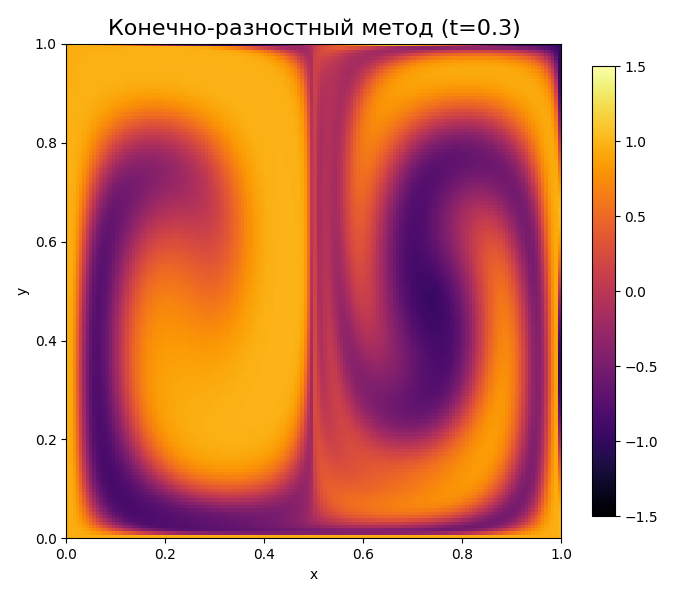
\includegraphics[width=\linewidth]{comparison_results/fdm_method_t_0.3.png}
    \end{minipage}
    \caption{Сравнение результатов в момент времени t=0.3. Слева — метод частиц, справа — конечно-разностный метод.}
    \label{fig:t03}
\end{figure}

% --- Сравнение для t=0.4 ---
\begin{figure}[H]
    \centering
    \begin{minipage}{0.49\textwidth}
        \centering
        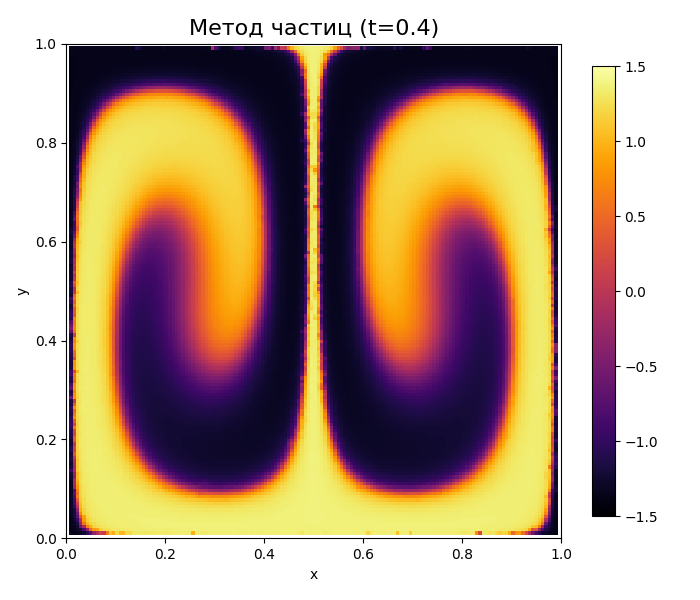
\includegraphics[width=\linewidth]{comparison_results/particle_method_t_0.4.png}
    \end{minipage}
    \hfill
    \begin{minipage}{0.49\textwidth}
        \centering
        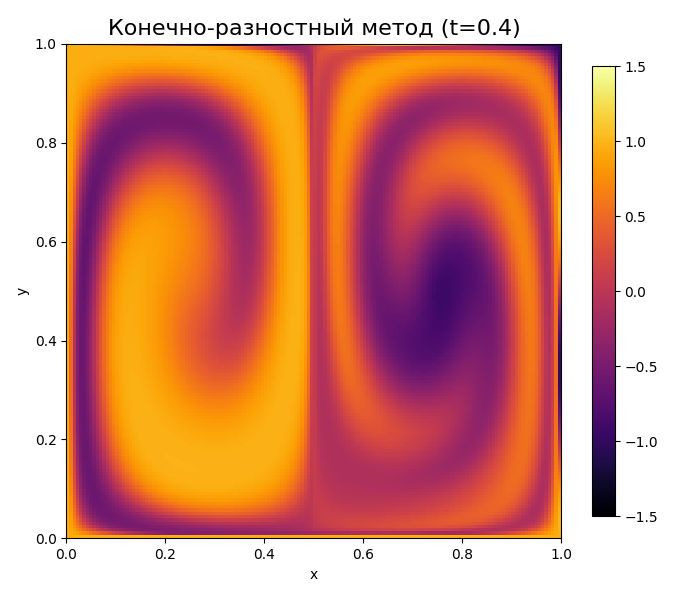
\includegraphics[width=\linewidth]{comparison_results/fdm_method_t_0.4.png}
    \end{minipage}
    \caption{Сравнение результатов в момент времени t=0.4. Слева — метод частиц, справа — конечно-разностный метод.}
    \label{fig:t04}
\end{figure}

\newpage

\subsection{Анализ результатов}
Визуальное сравнение результатов наглядно демонстрирует ключевые различия между двумя методами:

\paragraph{Четкость границ.} Метод частиц (левые графики на рисунках \ref{fig:t01}-\ref{fig:t04}) превосходно сохраняет резкость фронта концентрации на протяжении всего времени моделирования. Структура поля деформируется, но не "размывается".

\paragraph{Численная диффузия.} Конечно-разностный метод (правые графики) демонстрирует сильную численную диффузию. Уже на первом временном срезе (t=0.1) видно, как изначально резкая граница сглаживается. К концу моделирования (t=0.4) распределение становится значительно более размытым по сравнению с результатом метода частиц.

\paragraph{Сохранение формы.} Несмотря на размытие, оба метода корректно воспроизводят общую макроскопическую картину переноса — формирование характерной U-образной структуры, закручивающейся в два вихря. Это говорит о том, что оба подхода правильно моделируют адвекцию потока в целом.
Таким образом, численные эксперименты подтверждают теоретические свойства методов: лагранжев подход является более точным для решения задач чистого переноса, в то время как простой эйлеров подход, будучи проще в реализации на сетке, вносит существенные численные искажения в виде диффузии.

\newpage

\section{Вывод}
В данной работе был описан метод частиц для процесса переноса в стационарном поле скорости. Метод представляет собой систему двух дифференциальных уравнений перового порядка, которая описывает движение одной частицы. Описан алгоритм построения решения и написана программа, реализующая данный алгоритм. Результаты были визуализированы, а также интерполированием получено окончательное численное решение задачи.

\newpage

\section{Приложение}

\begin{minted}[fontsize=\small]{python}
import numpy as np
import matplotlib.pyplot as plt
import os

# =============================================================================
# 1. ОБЩИЕ ПАРАМЕТРЫ И ФУНКЦИИ
# =============================================================================
T_MAX = 0.4
COMPARE_TIMES = [0.1, 0.2, 0.3, 0.4]

NX, NY = 150, 150
NUM_PARTICLES = 30000

if not os.path.exists('comparison_results'):
    os.makedirs('comparison_results')

def u(x, y):
    return -np.pi * np.sin(2 * np.pi * x) * np.cos(np.pi * y)

def v(x, y):
    return 2 * np.pi * np.cos(2 * np.pi * x) * np.sin(np.pi * y)

# =============================================================================
# 2. РЕАЛИЗАЦИЯ МЕТОДА ЧАСТИЦ (ЛАГРАНЖЕВ ПОДХОД)
# =============================================================================
def run_particle_method(target_times):
    print("Запуск симуляции: Метод частиц...")
    from scipy.interpolate import griddata

    points = np.random.rand(NUM_PARTICLES, 2)
    concentrations = np.arctan((points[:, 1] - 0.5) / 0.1)
    
    dt = 0.001
    time = 0.0
    results = {}
    
    def velocity_field(p):
        return np.array([u(p[:, 0], p[:, 1]), v(p[:, 0], p[:, 1])]).T

    max_time_to_run = max(target_times)
    times_to_save = sorted(target_times)
    
    # ИСПРАВЛЕНИЕ: Добавляем небольшой буфер (dt/2) к условию цикла
    while time <= max_time_to_run + dt / 2:
        if times_to_save and time >= times_to_save[0]:
            current_save_time = times_to_save.pop(0)
            print(f"  Метод частиц: сохраняем срез на t={current_save_time:.1f}...")
            grid_x, grid_y = np.mgrid[0:1:complex(0, NX), 0:1:complex(0, NY)]
            interpolated_grid = griddata(points, concentrations, (grid_x, grid_y), method='linear')
            results[current_save_time] = interpolated_grid
        
        k1 = velocity_field(points)
        k2 = velocity_field(points + 0.5 * dt * k1)
        k3 = velocity_field(points + 0.5 * dt * k2)
        k4 = velocity_field(points + dt * k3)
        points += (dt / 6.0) * (k1 + 2 * k2 + 2 * k3 + k4)
        time += dt

    if times_to_save:

        save_time = times_to_save.pop(0)

        print(f"  Метод частиц: сохраняем срез на t={save_time:.1f}...")
        grid_x, grid_y = np.mgrid[0:1:complex(0, NX), 0:1:complex(0, NY)]
        interpolated_grid = griddata(points, concentrations, (grid_x, grid_y), method='linear')
        results[save_time] = interpolated_grid

    print("Метод частиц: симуляция завершена.")
    return results

# =============================================================================
# 3. РЕАЛИЗАЦИЯ КОНЕЧНО-РАЗНОСТНОГО МЕТОДА (ЭЙЛЕРОВ ПОДХОД)
# =============================================================================
def run_finite_difference_method(target_times, initial_C, U_grid, V_grid):
    print("Запуск симуляции: Конечно-разностный метод...")
    C = initial_C.copy()
    dx = 1.0 / (NX - 1)
    dy = 1.0 / (NY - 1)

    u_max, v_max = np.max(np.abs(U_grid)), np.max(np.abs(V_grid))
    dt = 0.5 / (u_max / dx + v_max / dy)
    
    time = 0.0
    results = {}
    times_to_save = sorted(target_times)
    max_time_to_run = max(target_times)
    
    while time <= max_time_to_run + dt / 2:
        if times_to_save and time >= times_to_save[0]:
            current_save_time = times_to_save.pop(0)
            print(f"  К-Р метод: сохраняем срез на t={current_save_time:.1f}...")
            results[current_save_time] = C.copy()

        C_old = C.copy()
        for i in range(1, NX - 1):
            for j in range(1, NY - 1):
                if U_grid[j, i] >= 0:
                    dCdx = (C_old[j, i] - C_old[j, i - 1]) / dx
                else:
                    dCdx = (C_old[j, i + 1] - C_old[j, i]) / dx
                if V_grid[j, i] >= 0:
                    dCdy = (C_old[j, i] - C_old[j - 1, i]) / dy
                else:
                    dCdy = (C_old[j + 1, i] - C_old[j, i]) / dy
                C[j, i] = C_old[j, i] - dt * (U_grid[j, i] * dCdx + V_grid[j, i] * dCdy)
        time += dt

    if times_to_save:
        save_time = times_to_save.pop(0)
        print(f"  К-Р метод: сохраняем срез на t={save_time:.1f}...")
        results[save_time] = C.copy()
    
        
    print("Конечно-разностный метод: симуляция завершена.")
    return results

# =============================================================================
# 4. ФУНКЦИЯ ДЛЯ СОХРАНЕНИЯ ОДИНОЧНОГО ГРАФИКА
# =============================================================================
def save_single_plot(data, title, filename):
    """Создает, настраивает и сохраняет один график."""
    fig, ax = plt.subplots(figsize=(7, 6))
    
    vmin, vmax = -1.5, 1.5
    cmap = 'viridis'
    
    im = ax.imshow(data.T, extent=(0, 1, 0, 1), origin='lower', cmap=cmap, vmin=vmin, vmax=vmax)
    ax.set_title(title, fontsize=16)
    ax.set_xlabel('x')
    ax.set_ylabel('y')
    
    fig.colorbar(im, ax=ax, shrink=0.85)
    
    plt.tight_layout()
    plt.savefig(filename)
    plt.close(fig) #
    print(f"Сохранено: {filename}")

# =============================================================================
# 5. ЗАПУСК И ВИЗУАЛИЗАЦИЯ
# =============================================================================
if __name__ == '__main__':
    x = np.linspace(0, 1, NX)
    y = np.linspace(0, 1, NY)
    X, Y = np.meshgrid(x, y)
    C_initial = np.arctan((Y - 0.5) / 0.1)
    U_grid = u(X, Y)
    V_grid = v(X, Y)

    # --- Запуск симуляций ---
    particle_results = run_particle_method(COMPARE_TIMES)
    fdm_results = run_finite_difference_method(COMPARE_TIMES, C_initial, U_grid, V_grid)

    os.makedirs('lab6/comparison_results', exist_ok=True)

    print("\nСохранение начального состояния...")
    save_single_plot(C_initial.T, 'Начальное состояние (t=0.0)', 'lab6/comparison_results/initial_state.png')

    
    print("\nСохранение результатов по временным срезам...")
    for t in COMPARE_TIMES:
        p_data = particle_results[t]
        p_title = f'Метод частиц (t={t:.1f})'
        p_filename = f'lab6/comparison_results/particle_method_t_{t:.1f}.png'
        save_single_plot(p_data, p_title, p_filename)
        
        fdm_data = fdm_results[t]
        fdm_title = f'Конечно-разностный метод (t={t:.1f})'
        fdm_filename = f'lab6/comparison_results/fdm_method_t_{t:.1f}.png'
        save_single_plot(fdm_data.T, fdm_title, fdm_filename)

    print("\nВсе файлы успешно созданы.")
\end{minted}


\end{document}


